\begin{frame}[allowframebreaks]{}
    \LARGE Normalizing Flow Models: \\[1.5ex] \textbf{\Large Real NVP - Real-valued Non-Volume Preserving}
\end{frame}

\begin{frame}[allowframebreaks]{Real NVP}
\textbf{RealNVP: Real-valued Non-Volume Preserving}
\begin{itemize}
    \item Enhancements over NICE:
    \begin{itemize}
        \item Introduces scaling in coupling layers:
        \begin{itemize}
            \item Partition the variables $z$ into two disjoint subsets.
            \item $x_{1:d} = z_{1:d}$
            \item $x_{d+1:n} = z_{d+1:n} \bigodot \exp\left(F(z_{1:d})\right) + H(z_{1:d})$, where $F$ and $H$ are neural networks.
        \end{itemize}
        \begin{figure}
            \centering
            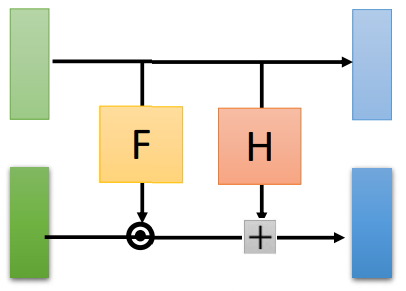
\includegraphics[height=0.4\textheight, width=\textwidth, keepaspectratio]{images/norm-flow/nfm_realnvp.png}
        \end{figure}
        \item Allows modeling of volume changes, increasing flexibility.
    \end{itemize}
    \framebreak
    \item \textbf{Benefits:}
    \begin{itemize}
        \item Efficient computation of the Jacobian determinant due to the triangular structure.
        \item Supports exact likelihood estimation and sampling.
    \end{itemize}
    \item \textbf{Implementation Details:}
    \begin{itemize}
        \item Alternating the roles of $z_{1:d}$ and $z_{d+1:n}$ across layers ensures all dimensions are transformed.
    \end{itemize}
    \item Coupling layers are composed together (with arbitrary partitions of variables in each layer).
    
\end{itemize}
\end{frame}

\begin{frame}{Real NVP - Results}
\begin{figure}
    \centering
    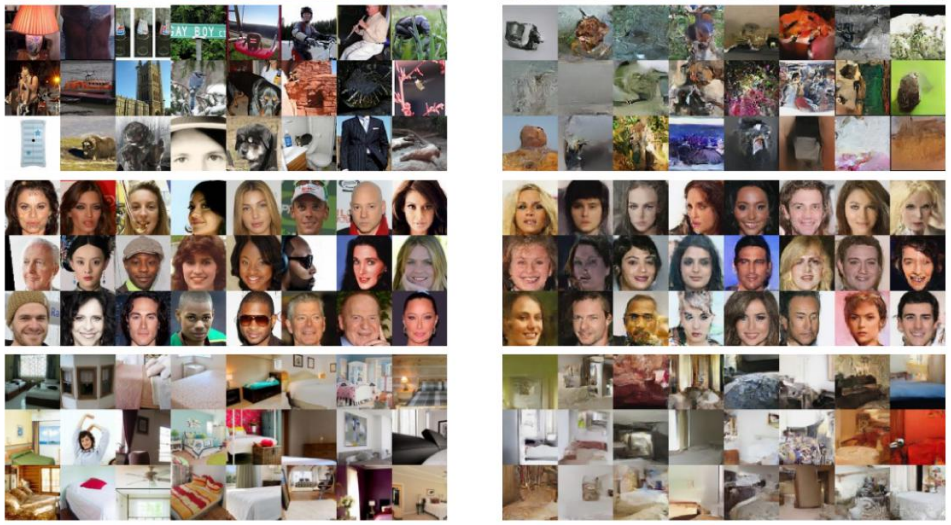
\includegraphics[height=0.8\textheight, width=\textwidth, keepaspectratio]{images/norm-flow/nfm_realnvp_results.png}
    \caption*{Real NVP generated samples}
\end{figure}
\end{frame}